\documentclass{article}
\setlength{\textwidth}{6.5in} \setlength{\textheight}{8.5in}
\setlength{\evensidemargin}{-.2in}
\setlength{\oddsidemargin}{-0.16in}
\usepackage{times}
\usepackage{hyperref}
\title{Sequential Probability Ratio Test by R}
\author{Behzad FallahiFard
\\ \href{mailto:behzadfalahifard@gmail.com}{behzadfalahifard@gmail.com}
\\ \\{\small Advisor: Dr. Aliakbar Rasekhi}\\ \small{Assistant Professor of Statistics}\\ {\small Tarbiat Modares University, Iran}
\\ \href{mailto:rasekhi@modares.ac.ir}{rasekhi@modares.ac.ir}}
\usepackage{Sweave}
\begin{document}
\maketitle
\Sconcordance{concordance:SPRT.tex:SPRT.Rnw:%
1 11 1 1 0 43 1 1 51 50 0 1 5 3 0 1 1 6 0 1 2 1 0 1 1 6 0 1 2 1 0 1 1 6 %
0 1 2 1 0 1 1 6 0 1 2 1 0 1 1 6 0 1 2 1 0 1 1 8 0 1 2 11 1 1 2 1 0 1 32 %
30 0 1 3 2 1 7 0 1 2 7 1}

\section{Abstract}
In this project, a function called \texttt{sprt} is presented which has performed statistical testing of a simple hypothesis ($H_0$) versus another simple hypothesis ($H_1$) using the SPRT method. Also, another function called \texttt{en.sprt} is designed to estimate the number of sampling steps for accepting $H_0$ or accepting $H_1$.
%%%%%%%%%%%%%%%%%%%%%%%%%%%%%%%%%%%%%%
\section{Introduction}
In Neyman-Pearson statistical tests, the probability of statistical errors depends on the number of observations. In other words, by changing the number of observations, the probability of statistical errors can also be altered. However, in such tests, we keep the number of observations constant and reduce the probability of statistical errors.


Neyman-Pearson tests, especially Uniform Most Powerful (UMP) tests, are obtained when we can change the probability of errors, and the sample size is fixed. But in sequential tests, some methods are used to optimize sample size based on fixed probability of type I ($\alpha$) and type II ($\beta$) errors. These tests are based on the likelihood ratio tests. In section 3 we formulate the SPRT method, and an example and corresponding R codes are provided. The section 4 addresses formulation of estimating SPRT sample size, and represents an example and  R codes.
%%%%%%%%%%%%%%%%%%%%%%%%%%%%%%%%%%%%%%%%%%%%%%%%%%%%%%%%%%%%
\section{Preliminaries}
Let $X_1,X_2,...$ be a sequence of independent and identically distributed random variables with the probability density function $f$. Suppose that $f_0$ and $f_1$ are two possible densities for $X_i$s. $f_0$ and $f_1$ are both related to continuous distributions or discreet distributions with the same support.\\
Consider the following problem of testing

\begin{eqnarray*}
H_0:f=f_0  &versus&  H_1:f=f_1
\end{eqnarray*}
%%%%%%%%%%%%%%%%%%%%%%%%%%%%%%%%%%%%%
{\bf Definition}
\[{R_m}({x_1},{x_2}, \ldots ,{x_m}) = \frac{{{f_1}({x_1},{x_2}, \ldots ,{x_m})}}{{{f_0}({x_1},{x_2}, \ldots ,{x_m})}} = \prod\limits_{i = 1}^m {\frac{{{f_1}({x_i})}}{{{f_0}({x_i})}}} ,\,\,\,m = 1,2,...\]
\\
Wald (1945) considered $A$ and $B$ such that $0 < B < 1 < A < \infty$ and proposed following steps to judge the hypotheses after observing the first observation, $X_1=x_1$.\\\\
%%%%%%%%%%%%%%%%%%%%%%%%%%%%%%%%%%%%%
{\bf Step ${\bf m}$, $m = 1,2,...$}\\
\begin{itemize}
\item
If ${R_m}({x_1},{x_2}, \ldots ,{x_m}) \ge A$, stop sampling and accept $H_0$.\\
\item
If ${R_m}({x_1},{x_2}, \ldots ,{x_m}) \le B$, stop sampling and accept $H_1$.\\
\item
If $B<{R_m}({x_1},{x_2}, \ldots ,{x_m}) < A$, continue sampling  and repeat the process for step $m+1$\\
\end{itemize}
For two constant values $A$ and $B$, the method described before is called Sequential Probability Ratio Test (SPRT); Which is also the "best" sequential method.
In the SPRT method, we show the sample size with the symbol $N$, which is a random variable. In this method, it is proved that sampling ends; we do not need infinite observation. A logical approximation for $A$ and $B$ can be as follows
\[A \approx \frac{{1 - \beta }}{\alpha }\,\,\,\,{\rm{\& }}\,\,B\, \approx \frac{\beta }{{1 - \alpha }}\]
%%%%%%%%%%%%%%%%%%%%%%%%%%%%%%%%%%%%%%%%
\subsection{Example 1}
Let $S F F S S S F S...$ be an independent sequence of Bernoulli distribution,
\[{f_\theta }(x) = {\theta ^x}{(1 - \theta )^{1 - x}},\,\,x = 0,1\] Consider the problem of SPR testing
\[{H_0}:\theta  = 0.3\,\,\,\,\,versus\,\,\,\,\,{H_1}:\theta  = 0.6\]
If the probability of type I and type II errors are 0.2 ($\alpha=\beta=0.2$). At what step is the sampling stopped, and how is the test decision made?
\subsection{Codes 1}
\begin{Schunk}
\begin{Sinput}
> # B.FalahiFard 
>  
> #                     sprt : Sequential Probability Ratio Test
>  
> # Basic concepts of mathematical statistics A.Parsian 2nd edition page:436
> # If 'xm' is the observed sample in step m:
> # fH0  : f( x1,x2,...,xm | H0 )
> # fH1  : f( x1,x2,...,xm | H1 )
> # alpha: type I Error
> # beta : type II Error
> # R[m] = f( x1,x2,...,xm | H1 )/f( x1,x2,...,xm | H0 )
>  
> sprt<-function(fH0,fH1,alpha,beta){ 
+ A  <-(1-beta)/alpha      
+ B  <- beta/(1-alpha)   
+ f1 <-fH1               
+ f0 <-fH0
+ cp1<- cumprod(f1)     # If B < R[m] <A then countinue sampling. 
+ cp0<- cumprod(f0)     # If R[m] > A then H0 is rejceted by N=m observation.
+ m<- length(cp1)       # If R[m] < B then H0 is accepted by N=m observation.
+ R<- rep(0,m)
+ R<-cp1/cp0
+ y<- R
+ x<- rep(1:m)
+  
+ if(R[m]>B & R[m]<A){
+  
+ cat("\n","    B <  R","[",m,"]",
+ "< A    ","\n","",B,"<",R[m],"<",A,"   -->",
+ " Countinue sampling.","\n","\n")}
+  
+ else if(R[m]>A)
+ cat("\n","R","[",m,"]","> A    ","\n",R[m],">",A,"      -->",
+ " Rejcet H0.Finished","\n","\n")
+   
+ else cat("\n","B >","R","[",m,"]","\n",B,">",R[m],"       -->",
+ " Accept H0.Finished","\n","\n")
+  
+ if(R[m]<B | R[m]>A) {
+ plot(1,R[1],type="o",xlim=c(0,m),ylim=c(0,A+3),xlab="N",
+ ylab=expression(R[N]), main=expression('curve '(N,R[N])));
+  
+ u<-c(0,0,m,m+100);v<-c(0,B,B,0);polygon(u,v,col='green');
+ z<-c(A,A+100,A+100,A);polygon(u,z,col='7');
+  
+ lines(x,y,type="o",lwd=2);
+ abline(h=A,col='red');abline(h=B,col='red');
+ text(m/2,A+1.5,"Rejcet H0",col='blue',lwd=2);
+ text(m/2,B/2,"Accept Ho",col='blue',lwd=2);
+ }}
> #__________________________________________________ Solve 
> # z=(1,0,0,1,1,1,0,1,1, ... )
> #---------------------------------------------------Step 1:
> x<-c(1)
> sprt(dbinom(x,1,0.3),dbinom(x,1,0.6),0.2,0.2)
\end{Sinput}
\begin{Soutput}
     B <  R [ 1 ] < A     
  0.25 < 2 < 4    -->  Countinue sampling. 
\end{Soutput}
\begin{Sinput}
> #---------------------------------------------------Step 2:
> x<-c(1,0)
> sprt(dbinom(x,1,0.3),dbinom(x,1,0.6),0.2,0.2)
\end{Sinput}
\begin{Soutput}
     B <  R [ 2 ] < A     
  0.25 < 1.142857 < 4    -->  Countinue sampling. 
\end{Soutput}
\begin{Sinput}
> #---------------------------------------------------Step 3:
> x<-c(1,0,0)
> sprt(dbinom(x,1,0.3),dbinom(x,1,0.6),0.2,0.2)
\end{Sinput}
\begin{Soutput}
     B <  R [ 3 ] < A     
  0.25 < 0.6530612 < 4    -->  Countinue sampling. 
\end{Soutput}
\begin{Sinput}
> #---------------------------------------------------Step 4:
> x<-c(1,0,0,1)
> sprt(dbinom(x,1,0.3),dbinom(x,1,0.6),0.2,0.2)
\end{Sinput}
\begin{Soutput}
     B <  R [ 4 ] < A     
  0.25 < 1.306122 < 4    -->  Countinue sampling. 
\end{Soutput}
\begin{Sinput}
> #---------------------------------------------------Step 5:
> x<-c(1,0,0,1,1)
> sprt(dbinom(x,1,0.3),dbinom(x,1,0.6),0.2,0.2)
\end{Sinput}
\begin{Soutput}
     B <  R [ 5 ] < A     
  0.25 < 2.612245 < 4    -->  Countinue sampling. 
\end{Soutput}
\begin{Sinput}
> #---------------------------------------------------Step 6:
> x<-c(1,0,0,1,1,1)
> sprt(dbinom(x,1,0.3),dbinom(x,1,0.6),0.2,0.2)
\end{Sinput}
\begin{Soutput}
 R [ 6 ] > A     
 5.22449 > 4       -->  Rejcet H0.Finished 
\end{Soutput}
\end{Schunk}
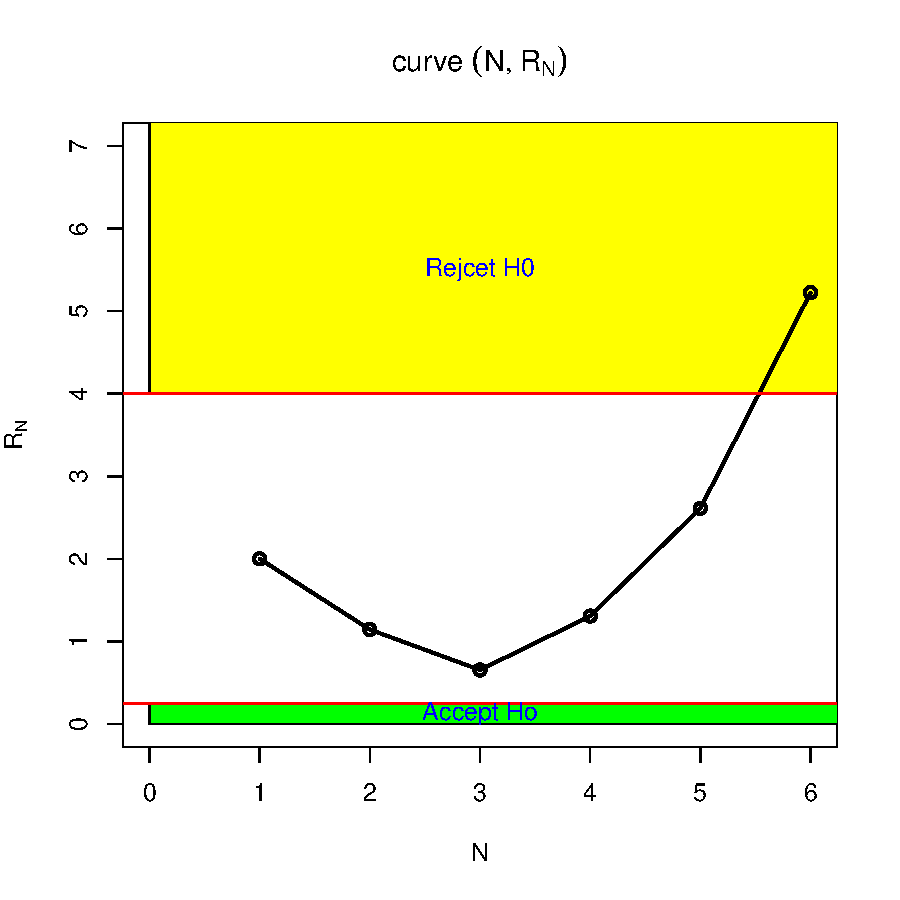
\includegraphics{SPRT-001}
\section{Expectation of Sampling Steps}
In many cases, the SPR test requires, on average, only half of the sample needed for the most powerful test (MPT). In other words, for each given pair $(\alpha, \beta)$, the sample size required in the sequential analysis is half of the sample size needed for the analysis based on fixed sample size; Therefore, we want to calculate the expected number of samples required under $H_0$ and $H_1$ in this method.
Suppose $X_1,X_2,...$ is a sequence of independent random variables with the same probability density function (or probability function) $f$. We want to perform the following test using the SPRT method.\\\\
If $a = \ln (A) = \ln (\frac{{1 - \beta }}{\alpha }),\,\,b = \ln (B) = \ln (\frac{\beta }{{1 - \alpha }})$, and ${z_1} = \ln (\frac{{{f_1}({X_1})}}{{{f_0}({X_1})}})$ then:
\[{E_{{H_0}}}(N) \approx \frac{{a\alpha  + b(1 - \alpha )}}{{{E_{{H_0}}}({z_1})}}\,\,\,\,\,{\rm{\& }}\,\,\,\,{E_{{H_1}}}(N) \approx \frac{{b\beta  + a(1 - \beta )}}{{{E_{{H_1}}}({z_1})}}\]
\\for ${{E_{{H_0}}}({z_1}) = 0}$ or ${{E_{{H_1}}}({z_1}) = 0}$ :
\[{E_{{H_i}}}(N) \approx  - \frac{{ab}}{{{E_{{H_i}}}(z_1^2)}},\,\,\,i = 0,1\]
%%%%%%%%%%%%%%%%%%%%%%%%%%%%%%%%%%%%%%%%%%%%%%%%%%%%%%%%%%%%%%%%%%%%%%%%%%%%
\subsection{Example 2}
Let $X_1,X_2,...$ is a sequence of random variables of normal distribution with mean parameter $\theta$ and variance parameter ${\sigma ^2} = 100$. If $\alpha=0.01$, and $\beta=0.05$ consider the problem of SPR testing 
%%%%%%%%%%%%%%%%%%%%%%%%%%%%%%%%%%%%%%%%%%%%%%%%%%%%%%%%%%%%%%%%%%%%%%%%%%%%
\subsection{Codes 2}
\begin{Schunk}
\begin{Sinput}
> rm(list=ls())
> # dname0: we substitute letter "d" before R name of distribution H0.
> # p0 ::::: the vector of parameters under H0.
> # x0     : the vector of simulated data under Ho.
> # dname1: we substitute letter "d" before R name of distribution H1.
> # p1 ::::: the vector of parameters under H1.
> # x1     : the vector of simulated data under H1.
> # alpha::: the probability of Type I error.
> # beta   : the probability of Type II error.
> 
> en.sprt<- function(dname0,p0,x0,dname1,p1,x1,alpha,beta){
+   a<-   log((1-beta)/alpha)
+   b<-   log(beta/(1-alpha))
+   if(length(p0)==3){
+     zH0<- log(dname1(x0,p1[1],p1[2],p1[3])/dname0(x0,p0[1],p0[2],p0[3]));
+     zH1<- log(dname1(x1,p1[1],p1[2],p1[3])/dname0(x1,p0[1],p0[2],p0[3]))}
+   
+   else if(length(p0)==2){
+     zH0<- log(dname1(x0,p1[1],p1[2])/dname0(x0,p0[1],p0[2]));
+     zH1<- log(dname1(x1,p1[1],p1[2])/dname0(x1,p0[1],p0[2]))}
+   
+   else if(length(p0)==1){
+     zH0<- log(dname1(x0,p1[1])/dname0(x0,p0[1]));
+     zH1<- log(dname1(x1,p1[1])/dname0(x1,p0[1]))}
+   
+   if(mean(zH0)==0)EH0N<- -(a*b)/mean((zH0)^2)
+   else EH0N<- (a*alpha +b*(1-alpha))/mean(zH0)
+   if(mean(zH1)==0)EH1N<- -(a*b)/mean((zH1)^2)
+   else EH1N<- (a*(1-beta) + b*beta)/mean(zH1)
+   cat("\n","The expected sample size for accepting H0 :",EH0N,"\n",
+       "The expected sample size for accepting H1 :",EH1N,"\n","\n")
+ }
> x0<- rnorm(10000,100,10)
> x1<- rnorm(10000,105,10)
> en.sprt(dnorm,c(100,10),x0,dnorm,c(105,10),x1,0.01,0.05)
\end{Sinput}
\begin{Soutput}
 The expected sample size for accepting H0 : 23.54244 
 The expected sample size for accepting H1 : 30.43614 
\end{Soutput}
\end{Schunk}
\newpage
\section{References}
Mood. A, Graybill. F, Boes. D. (1973) {\it Introduction to the Theory of Statistics}. McGraw-Hill.\\\\
Parsian. A. (2009). {\it Basic Concepts of Mathematical Statistics}. Isfahan University of Technology.\\\\
Wald. A (1945). Sequential Tests of Statistical Hypotheses. {\it Annals of Mathematical Statistics}. 16 (2): 117-186.\\\\
\end{document}


